\chapter{Liver Cirrhosis}
\label{applications-efx_country_level}

Besides explaining the bias of noisy measurement as discussed in Chapter \ref{applications-efx_study_level}, fixed effects can also increase the accuracy of out-of-sample predictions.  By modeling the relationship between the epidemiologic parameter of interest and an explanatory covariate, extrapolation can predict epidemiologic parameters in areas where no epidemiologic parameter measurements are available but covariate data are.  Few regions have epidemiologic measurements for liver cirrhosis.  However, by using the natural log of the age-standardized cirrhosis death rate as a country-level covariate to predict out-of-sample, it is possible to estimate the prevalence of cirrhosis.

As the result of chronic liver injury, liver cirrhosis is an advanced stage of liver scarring.  Cirrhosis is the end stage of any chronic liver disease, with the most common causes being alcoholic liver disease and hepatitis B and C.  Asymptomatic during the early stages of the disease, compensated cirrhosis may go undetected until complications develop.  The diagnostic gold standard for cirrhosis is a liver biopsy.  Complications such as portal hypertension, jaundice, ascites, gastrointestinal bleeding and liver dysfunction mark the progression from compensated to decompensated cirrhosis.  Irreversible, cirrhosis management is the prevention, control and treatment of cirrhosis complications, with liver transplantation being the ultimate treatment.  Without a liver transplant, cirrhosis mortality is very high \cite{garcia-tsao_management_2009, d'amico_natural_2006, schuppan_liver_2008}.

Systematic review yielded prevalence and cause-specific mortality rate estimates from 4 (of 21 possible) regions.  Given the difficulty in cirrhosis diagnosis, it is assumed this data represents decompensated cirrhosis and the following analysis focuses on the decompensated phase of the disease, assuming almost all prevalent cases lead to death.

    \begin{figure}[h]
        \begin{center}
            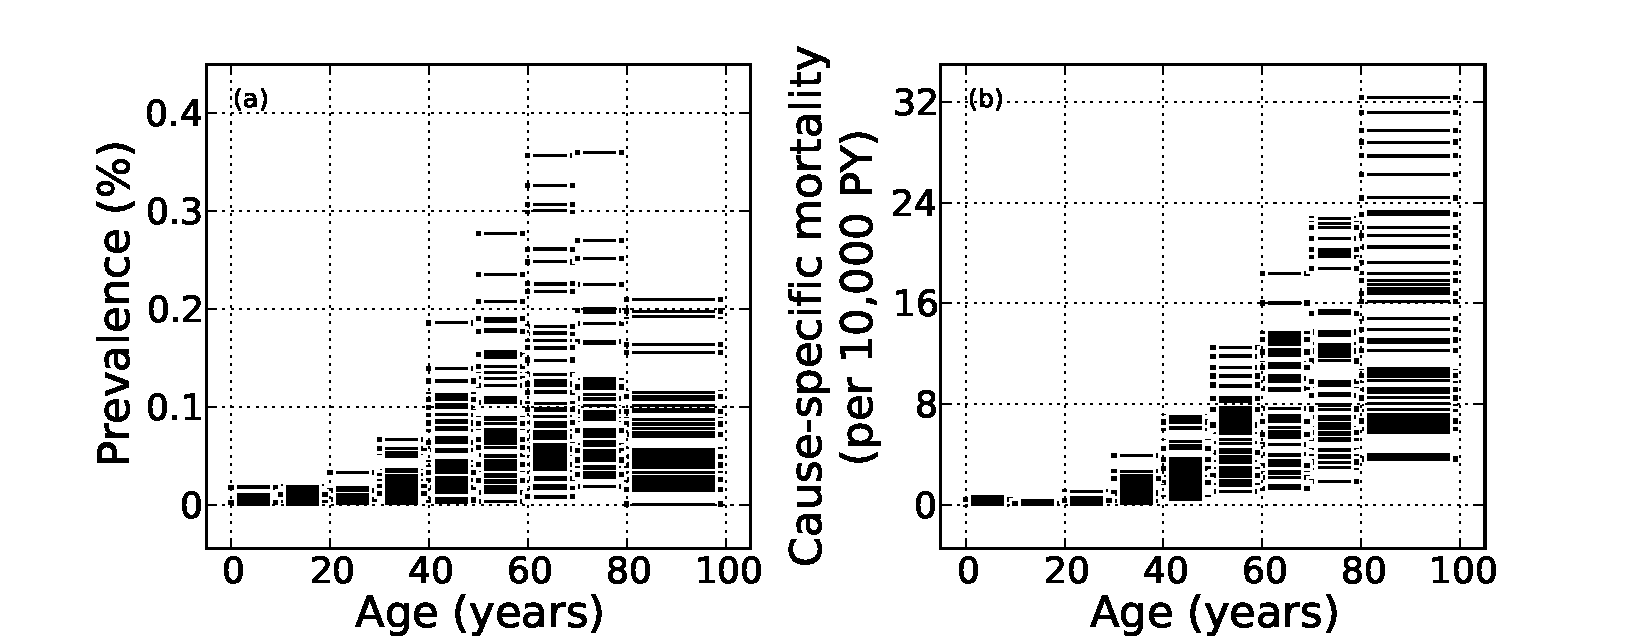
\includegraphics[width=\textwidth]{cirrhosis-data.pdf}
            \caption{Available global data for cirrhosis prevalence (a) and cause-specific mortality (b).}
            \label{fig:app-cirrhosis data}
        \end{center}
    \end{figure}

Since cirrhosis is so deadly, it is a reasonable assumption that regions with increased deaths from cirrhosis also have increased cirrhosis prevalence.  Figure \ref{fig:app-cirrhosis asp} shows the relationship between cirrhosis prevalence and the age-standardized death rate of cirrhosis.

    \begin{figure}[h]
        \begin{center}
            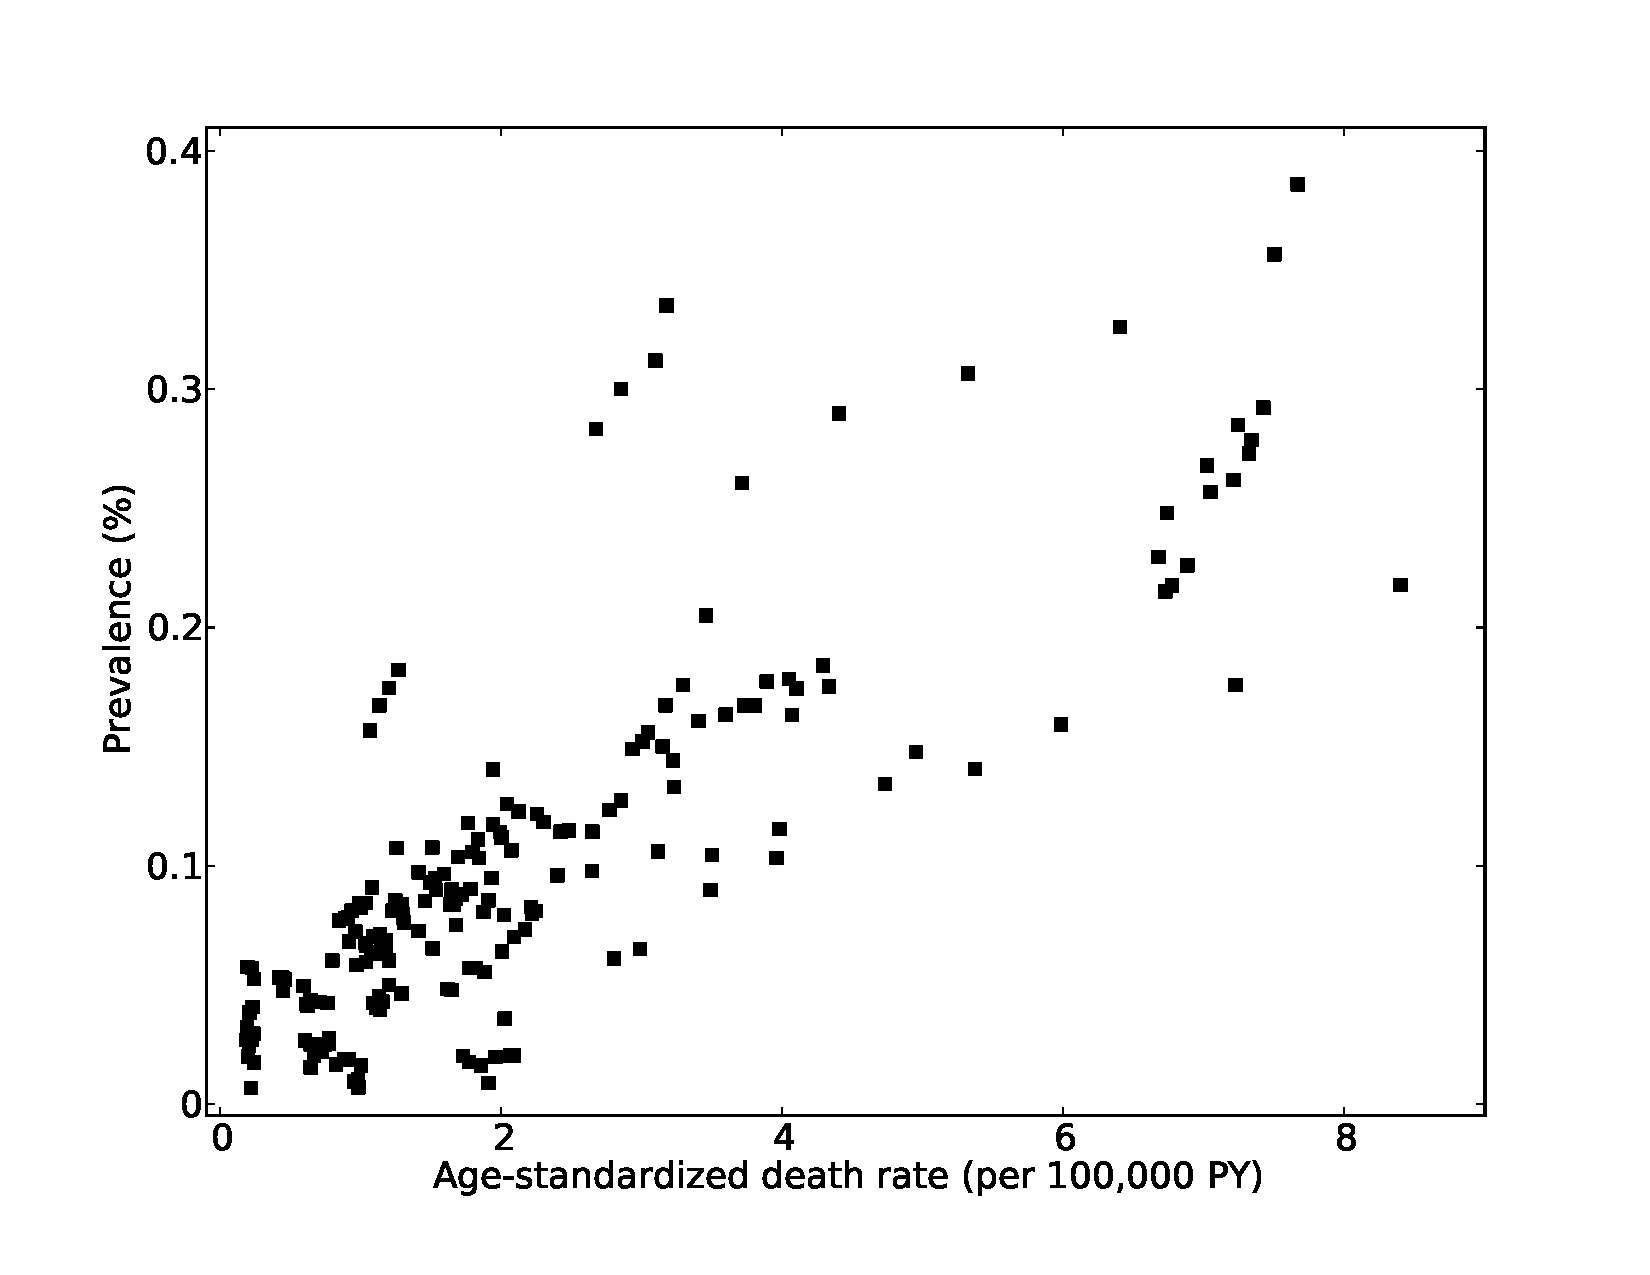
\includegraphics[width=\textwidth]{cirrhosis-lnASDR_v_prev.pdf}
            \caption{Relationship between cirrhosis prevalence and the natural log of the age-standardized death rate of cirrhosis.}
            \label{fig:app-cirrhosis asp}
        \end{center}
    \end{figure}

In regions with no cirrhosis data, estimates of the age-standardized cirrhosis death rate may be used as an explanatory covariate to estimate cirrhosis prevalence.  By borrowing strength from the mortality estimates to inform the incidence estimates, cirrhosis prevalence can be estimated for regions without data as shown in Figure \ref{fig:app-cirrhosis prev est}.

    \begin{figure}[h]
        \begin{center}
            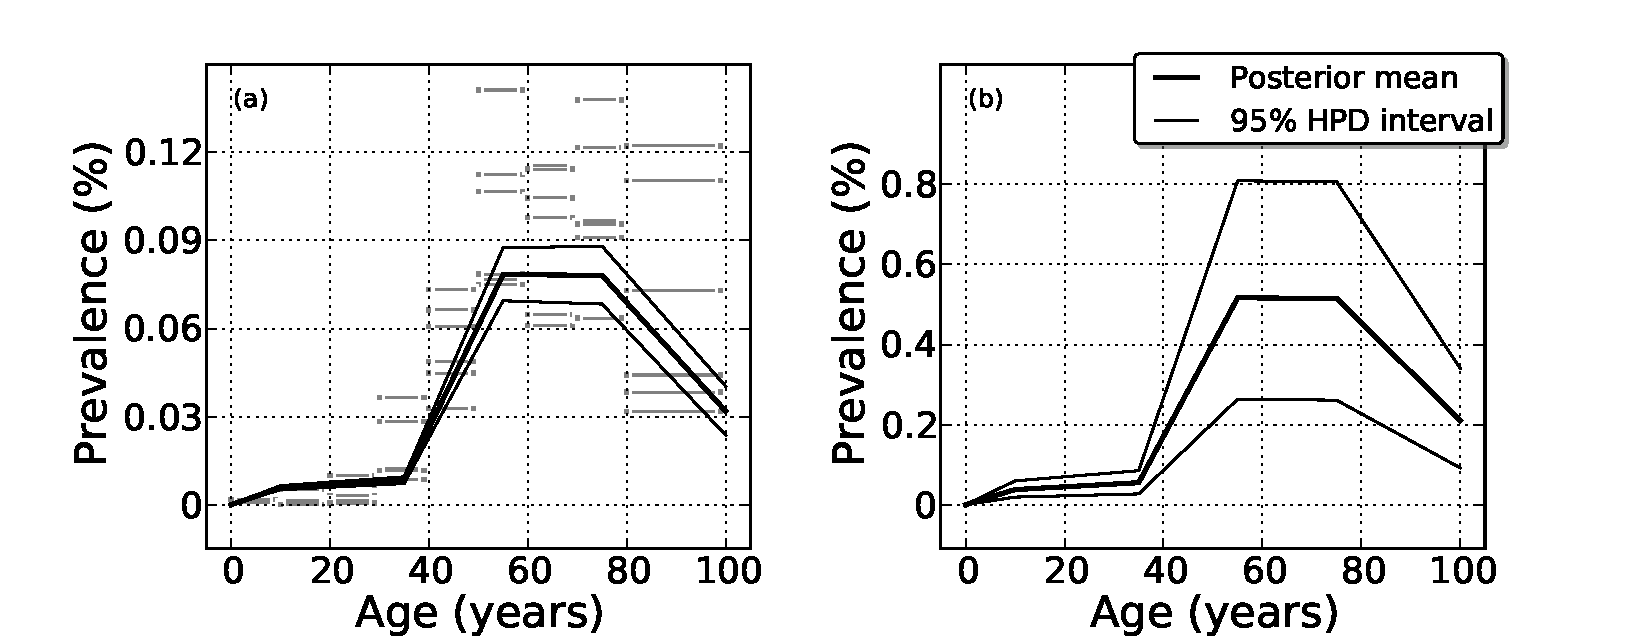
\includegraphics[width=\textwidth]{cirrhosis-prev_est.pdf}
            \caption{Cirrhosis prevalence estimates Chinese (a) and Egyptian (b) males in 2005.}
            \label{fig:app-cirrhosis prev est}
        \end{center}
    \end{figure}
